\documentclass[11pt,a4paper]{article}

\usepackage[T1]{fontenc}
\usepackage[utf8]{inputenc}
\usepackage[provide=*,italian]{babel}
\usepackage{lmodern}
\usepackage{microtype}
\usepackage{geometry}
\geometry{margin=2.5cm}
\usepackage{amsmath,amssymb,amsthm,mathtools}
\usepackage{booktabs,array,longtable}
\usepackage{blkarray}
\usepackage{xcolor}
\usepackage{enumitem}
\usepackage{tikz}
\usetikzlibrary{arrows.meta,positioning,calc}
\usepackage[most]{tcolorbox}
\usepackage{listings}
\usepackage{hyperref}
\usepackage{fancyhdr}

\definecolor{sapienzared}{RGB}{130,0,36}
\definecolor{softred}{RGB}{249,241,243}
\definecolor{softblue}{RGB}{239,246,252}
\definecolor{softgray}{RGB}{245,245,245}
\definecolor{codegreen}{RGB}{25,110,65}

\hypersetup{
  colorlinks=true,
  linkcolor=sapienzared,
  urlcolor=sapienzared,
  pdftitle={Reti di flusso e matrice di incidenza},
  pdfauthor={Giampaolo Liuzzi}
}

\pagestyle{fancy}
\fancyhf{}
\fancyhead[L]{\small Ottimizzazione su Reti}
\fancyhead[R]{\small Capitolo 4}
\fancyfoot[C]{\thepage}
\renewcommand{\headrulewidth}{0.4pt}

\newtheorem{definition}{Definizione}[section]
\newtheorem{theorem}[definition]{Teorema}
\newtheorem{proposition}[definition]{Proposizione}
\newtheorem{observation}[definition]{Osservazione}

\newtcolorbox{learningbox}{
  colback=softred,colframe=sapienzared,
  title=Obiettivi di apprendimento,fonttitle=\bfseries,
  boxrule=0.8pt,arc=1.5mm
}
\newtcolorbox{examplebox}[1]{
  colback=softblue,colframe=blue!55!black,
  title=#1,fonttitle=\bfseries,
  boxrule=0.7pt,arc=1.5mm
}
\newtcolorbox{warningbox}{
  colback=yellow!9,colframe=orange!65!black,
  title=Attenzione alla convenzione dei segni,fonttitle=\bfseries,
  boxrule=0.7pt,arc=1.5mm
}
\newtcolorbox{networkxbox}{
  colback=softgray,colframe=black!55,
  title=Collegamento con Python/NetworkX,fonttitle=\bfseries,
  boxrule=0.7pt,arc=1.5mm
}

\lstdefinestyle{python}{
  language=Python,
  basicstyle=\ttfamily\small,
  keywordstyle=\color{blue!65!black}\bfseries,
  commentstyle=\color{codegreen},
  stringstyle=\color{sapienzared},
  backgroundcolor=\color{softgray},
  frame=single,
  rulecolor=\color{black!25},
  showstringspaces=false,
  breaklines=true,
  columns=fullflexible
}

\newcommand{\R}{\mathbb{R}}
\newcommand{\Z}{\mathbb{Z}}
\newcommand{\V}{\mathcal{V}}
\newcommand{\E}{\mathcal{E}}
\newcommand{\deltaout}{\delta^{+}}
\newcommand{\deltain}{\delta^{-}}

\begin{document}
\pagenumbering{roman}

\begin{titlepage}
  \centering
  \vspace*{1.6cm}
  {\color{sapienzared}\rule{\textwidth}{1.2pt}}\\[1.1cm]
  {\Large Ottimizzazione su Reti}\\[0.35cm]
  {\huge\bfseries Capitolo 4}\\[0.45cm]
  {\LARGE\bfseries Reti di flusso e matrice di incidenza}\\[1.1cm]
  {\color{sapienzared}\rule{0.72\textwidth}{0.8pt}}\\[1.1cm]
  {\large Corso di Laurea Magistrale in Ingegneria Gestionale}\\[0.25cm]
  {\large Sapienza Università di Roma}\\[1.2cm]
  {\large Giampaolo Liuzzi}\\[0.25cm]
  {\normalsize Dipartimento di Ingegneria Informatica, Automatica e Gestionale}\\[2cm]
  \vfill
  {\small Versione preliminare per uso didattico}
\end{titlepage}

\tableofcontents
\newpage
\pagenumbering{arabic}

\begin{learningbox}
Al termine del capitolo lo studente dovrebbe essere in grado di:
\begin{itemize}[nosep]
  \item passare da un grafo orientato a una rete di flusso;
  \item costruire la matrice di incidenza nodo-arco secondo una convenzione fissata;
  \item scrivere e interpretare i vincoli di bilancio $Ax=b$;
  \item distinguere nodi di offerta, domanda e transito;
  \item verificare l'ammissibilità di un flusso rispetto a bilanci e capacità;
  \item riconoscere le proprietà strutturali della matrice di incidenza che saranno utilizzate dal simplesso su reti;
  \item rappresentare e controllare una piccola rete mediante Python e NetworkX.
\end{itemize}
\end{learningbox}

\section{Dal grafo alla rete di flusso}

Un grafo orientato descrive quali collegamenti sono possibili e in quale direzione possono essere percorsi. Una \emph{rete di flusso} aggiunge informazioni quantitative: quantità disponibili o richieste nei nodi, costi di utilizzo degli archi e limiti alle quantità che possono attraversarli.

Nel seguito indichiamo con
\[
  G=(\V,\E)
\]
un grafo orientato finito, dove $\V=\{1,\ldots,n\}$ è l'insieme dei nodi ed $\E\subseteq \V\times\V$ è l'insieme degli archi. Il numero degli archi è indicato con $m=|\E|$. A ogni arco $(i,j)\in\E$ associamo una variabile
\[
  x_{ij}=\text{quantità di flusso inviata dal nodo $i$ al nodo $j$}.
\]

\begin{definition}[Rete di flusso]
Una rete di flusso è un grafo orientato $G=(\V,\E)$ al quale sono associati:
\begin{itemize}[nosep]
  \item un bilancio $b_i\in\R$ per ogni nodo $i\in\V$;
  \item un costo unitario $c_{ij}\in\R$ per ogni arco $(i,j)\in\E$;
  \item un limite inferiore $\ell_{ij}\in\R$ e una capacità superiore $u_{ij}\in\R\cup\{+\infty\}$ per ogni arco, con $\ell_{ij}\le u_{ij}$.
\end{itemize}
\end{definition}

La quantità $c_{ij}$ misura il costo sostenuto per ogni unità di flusso sull'arco $(i,j)$. I limiti impongono
\[
  \ell_{ij}\le x_{ij}\le u_{ij}.
\]
Nei primi esempi useremo spesso $\ell_{ij}=0$. Quando $u_{ij}=+\infty$, l'arco è detto non capacitato.

\subsection{Archi entranti e uscenti}

Per ogni nodo $i\in\V$ definiamo
\begin{align*}
  \deltaout(i)&=\{(i,j)\in\E\}, &&\text{insieme degli archi uscenti da $i$},\\
  \deltain(i)&=\{(j,i)\in\E\}, &&\text{insieme degli archi entranti in $i$}.
\end{align*}
Il flusso totale uscente e quello entrante sono quindi
\[
  \sum_{(i,j)\in\deltaout(i)}x_{ij}
  \qquad\text{e}\qquad
  \sum_{(j,i)\in\deltain(i)}x_{ji}.
\]

\subsection{Offerte, domande e nodi di transito}

Adottiamo per tutte le dispense la convenzione utilizzata in NetworkX e nelle trasparenze del corso:
\[
\boxed{
  b_i>0\;\Longleftrightarrow\;\text{il nodo $i$ richiede un'entrata netta di $b_i$ unità}
}
\]
e pertanto il vincolo di bilancio nel nodo $i$ è
\begin{equation}\label{eq:balance}
  \sum_{(j,i)\in\deltain(i)}x_{ji}
  -\sum_{(i,j)\in\deltaout(i)}x_{ij}=b_i.
\end{equation}
Ne segue che:
\begin{itemize}
  \item se $b_i>0$, il nodo è un nodo di \emph{domanda};
  \item se $b_i<0$, il nodo è un nodo di \emph{offerta};
  \item se $b_i=0$, il nodo è un nodo di \emph{transito}.
\end{itemize}

\begin{warningbox}
In alcuni testi si usa la convenzione opposta: $b_i>0$ identifica un'offerta e il bilancio è scritto come flusso uscente meno flusso entrante. Le due scelte sono equivalenti, ma non devono essere mescolate. Nelle presenti dispense useremo sempre \emph{entrante meno uscente uguale a $b_i$}, in accordo con NetworkX.
\end{warningbox}

\begin{observation}
Sommando le equazioni di bilancio su tutti i nodi, ogni variabile $x_{ij}$ compare una volta con segno negativo, nel nodo di origine $i$, e una volta con segno positivo, nel nodo di destinazione $j$. Pertanto, una condizione necessaria per l'esistenza di un flusso ammissibile è
\begin{equation}\label{eq:globalbalance}
  \sum_{i\in\V} b_i=0.
\end{equation}
Questa condizione esprime l'uguaglianza tra offerta complessiva e domanda complessiva. In presenza di capacità, non è in generale sufficiente.
\end{observation}

\section{La matrice di incidenza nodo-arco}

Fissiamo un ordinamento dei nodi e degli archi. La matrice di incidenza consente di scrivere simultaneamente tutte le equazioni di bilancio.

\begin{definition}[Matrice di incidenza]
La matrice di incidenza nodo-arco di un grafo orientato $G=(\V,\E)$ è la matrice $A\in\R^{n\times m}$ i cui elementi sono
\[
  a_{ik}=\begin{cases}
  -1, & \text{se l'arco $k$ esce dal nodo $i$},\\
  +1, & \text{se l'arco $k$ entra nel nodo $i$},\\
  0,  & \text{altrimenti}.
  \end{cases}
\]
Equivalentemente, se la colonna $k$ corrisponde all'arco $(p,q)$, essa contiene $-1$ nella riga $p$, $+1$ nella riga $q$ e zero in tutte le altre righe.
\end{definition}

Ogni colonna di $A$ contiene dunque esattamente due elementi non nulli, uno uguale a $+1$ e uno uguale a $-1$.

\subsection{Un primo esempio}

Consideriamo la rete in Figura~\ref{fig:smallnetwork}, con archi ordinati come
\[
  e_1=(1,2),\quad e_2=(1,3),\quad e_3=(2,3),\quad e_4=(2,4),\quad e_5=(3,4).
\]

\begin{figure}[ht]
\centering
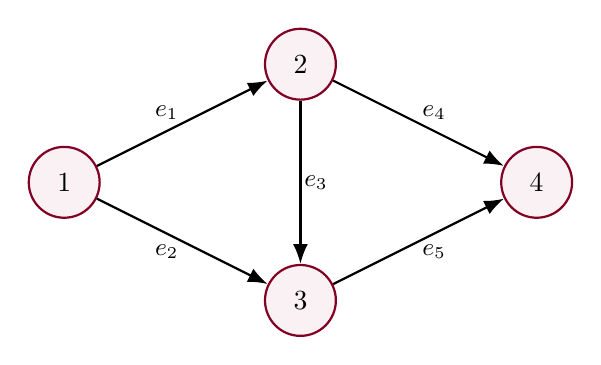
\begin{tikzpicture}[
  node/.style={circle,draw=sapienzared,thick,fill=softred,minimum size=9mm},
  arc/.style={-{Latex[length=2.5mm]},thick},
  lab/.style={font=\small,fill=white,inner sep=1pt}
]
\node[node] (n1) at (0,1.5) {1};
\node[node] (n2) at (3,3) {2};
\node[node] (n3) at (3,0) {3};
\node[node] (n4) at (6,1.5) {4};
\draw[arc] (n1) -- node[lab,above left] {$e_1$} (n2);
\draw[arc] (n1) -- node[lab,below left] {$e_2$} (n3);
\draw[arc] (n2) -- node[lab,right] {$e_3$} (n3);
\draw[arc] (n2) -- node[lab,above right] {$e_4$} (n4);
\draw[arc] (n3) -- node[lab,below right] {$e_5$} (n4);
\end{tikzpicture}
\caption{Una piccola rete orientata.}
\label{fig:smallnetwork}
\end{figure}

La matrice di incidenza è
\begin{equation}\label{eq:Aexample}
A=
\begin{blockarray}{cccccc}
 & e_1 & e_2 & e_3 & e_4 & e_5\\
\begin{block}{c[ccccc]}
1 & -1 & -1 &  0 &  0 &  0\\
2 &  1 &  0 & -1 & -1 &  0\\
3 &  0 &  1 &  1 &  0 & -1\\
4 &  0 &  0 &  0 &  1 &  1\\
\end{block}
\end{blockarray}.
\end{equation}
La stessa matrice, senza intestazioni, è
\[
A=\begin{bmatrix}
-1&-1& 0& 0& 0\\
 1& 0&-1&-1& 0\\
 0& 1& 1& 0&-1\\
 0& 0& 0& 1& 1
\end{bmatrix}.
\]

\subsection{Bilanci in forma matriciale}

Introduciamo i vettori
\[
  x=(x_{e_1},\ldots,x_{e_m})^\top\in\R^m,
  \qquad
  b=(b_1,\ldots,b_n)^\top\in\R^n.
\]
Per costruzione, la componente $i$ del prodotto $Ax$ è il flusso entrante nel nodo $i$ meno il flusso uscente. Tutte le equazioni~\eqref{eq:balance} possono quindi essere scritte come
\begin{equation}\label{eq:Ax=b}
  \boxed{Ax=b.}
\end{equation}

Per la rete della Figura~\ref{fig:smallnetwork}, il sistema è
\begin{align*}
-x_{12}-x_{13} &= b_1,\\
x_{12}-x_{23}-x_{24} &= b_2,\\
x_{13}+x_{23}-x_{34} &= b_3,\\
x_{24}+x_{34} &= b_4.
\end{align*}

\section{Proprietà strutturali della matrice di incidenza}

Le proprietà di $A$ spiegano perché i problemi di flusso possano essere risolti mediante algoritmi specializzati particolarmente efficienti.

\subsection{Dipendenza delle equazioni di bilancio}

Poiché la somma degli elementi di ogni colonna di $A$ è nulla,
\[
  \boldsymbol{1}^\top A=0^\top.
\]
Le righe di $A$ sono quindi linearmente dipendenti. Se il grafo è connesso in senso debole, una sola equazione di bilancio è ridondante.

\begin{theorem}[Rango della matrice di incidenza]
Sia $G$ un grafo orientato con $n$ nodi e $q$ componenti connesse, ignorando l'orientamento degli archi. Allora
\[
  \operatorname{rank}(A)=n-q.
\]
In particolare, se $G$ è connesso, $\operatorname{rank}(A)=n-1$.
\end{theorem}

\begin{proof}
In ogni componente connessa la somma delle righe corrispondenti è nulla; esistono quindi almeno $q$ dipendenze lineari indipendenti. D'altra parte, in ciascuna componente si può scegliere un albero ricoprente. Eliminando una riga per componente, le colonne associate agli archi di tali alberi formano una matrice quadrata non singolare. Il rango è pertanto almeno $n-q$, e le due stime coincidono.
\end{proof}

\begin{observation}
Quando $G$ è connesso e $\sum_i b_i=0$, possiamo eliminare una qualsiasi riga di $A$ e la corrispondente componente di $b$. Il sistema ridotto contiene tutte le informazioni del sistema originale. Questa operazione sarà fondamentale nello studio delle basi del simplesso su reti.
\end{observation}

\subsection{Orientamento e struttura}

L'orientamento scelto per un arco determina il segno della corrispondente colonna. Invertire l'arco $(i,j)$ in $(j,i)$ equivale a moltiplicare quella colonna per $-1$. Le proprietà di rango e la struttura combinatoria non cambiano.

Con la convenzione adottata, la colonna associata all'arco $(i,j)$ produce nel vincolo duale l'espressione $y_j-y_i$. Nei capitoli sui cammini minimi questa scelta condurrà direttamente alle condizioni di Bellman $y_j-y_i\le c_{ij}$.

\subsection{Totale unimodularità}

\begin{theorem}
La matrice di incidenza nodo-arco di un grafo orientato è totalmente unimodulare: ogni sua sottomatrice quadrata ha determinante appartenente a $\{-1,0,1\}$.
\end{theorem}

Una conseguenza fondamentale, che useremo nei capitoli successivi, è la seguente.

\begin{proposition}[Integrità]
Se $b$, $\ell$ e $u$ sono interi e il poliedro
\[
  \{x\in\R^m: Ax=b,\ \ell\le x\le u\}
\]
è non vuoto, tutti i suoi vertici sono interi.
\end{proposition}

Pertanto, per ottenere un flusso intero non occorre imporre esplicitamente $x\in\Z^m$: la struttura della rete e l'integrità dei dati sono sufficienti. Questo fatto distingue molti problemi di flusso dai generici problemi di programmazione lineare intera.

\section{Flussi ammissibili}

\begin{definition}[Flusso ammissibile]
Un vettore $x\in\R^m$ è un flusso ammissibile se soddisfa
\[
  Ax=b,\qquad \ell\le x\le u.
\]
\end{definition}

La verifica di ammissibilità ha quindi due parti:
\begin{enumerate}
  \item verifica locale dei bilanci in tutti i nodi;
  \item verifica dei limiti inferiori e superiori su tutti gli archi.
\end{enumerate}

\subsection{Esempio completo}

Consideriamo ancora la rete della Figura~\ref{fig:smallnetwork} e poniamo
\[
  b=\begin{bmatrix}-5&0&0&5\end{bmatrix}^{\top},
  \qquad \ell=0,
\]
con capacità
\[
  u=\begin{bmatrix}4&3&2&4&4\end{bmatrix}^{\top}.
\]
Il vettore
\[
  x=\begin{bmatrix}3&2&1&2&3\end{bmatrix}^{\top}
\]
è ammissibile. Infatti,
\[
Ax=
\begin{bmatrix}
 -3-2\\
3-1-2\\
2+1-3\\
2+3
\end{bmatrix}
=
\begin{bmatrix}-5\\0\\0\\5\end{bmatrix}=b,
\]
e tutte le componenti di $x$ rispettano $0\le x\le u$.

Il vettore
\[
  \widehat{x}=\begin{bmatrix}4&1&2&1&3\end{bmatrix}^{\top}
\]
rispetta le capacità, ma non i bilanci: nel nodo 2 si ha $4-2-1=1$, mentre nel nodo 4 si ha $1+3=4$. Pertanto $\widehat{x}$ non è ammissibile. Si osservi inoltre che, anche quando $b$ è fissato, la rete può ammettere più flussi ammissibili distinti.

\subsection{La condizione globale non è sufficiente}

Supponiamo che l'unico arco tra un nodo di offerta $s$ con $b_s=-10$ e un nodo di domanda $t$ con $b_t=10$ abbia capacità $u_{st}=7$. Vale $b_s+b_t=0$, ma nessun flusso può trasferire le dieci unità richieste. Le capacità e la topologia della rete possono dunque impedire l'ammissibilità anche quando la rete è globalmente bilanciata.

\section{Limiti inferiori e trasformazione dei bilanci}

Un limite inferiore positivo impone che una quantità minima attraversi un arco. Esso può essere eliminato mediante un cambio di variabili. Poniamo
\[
  y_{ij}=x_{ij}-\ell_{ij}.
\]
Allora $0\le y_{ij}\le u_{ij}-\ell_{ij}$ e
\[
  A(y+\ell)=b
  \quad\Longleftrightarrow\quad
  Ay=b-A\ell.
\]
Il problema con limiti inferiori $\ell$ è quindi trasformato in un problema con limiti inferiori nulli e nuovo vettore dei bilanci
\begin{equation}
  b'=b-A\ell.
\end{equation}

\begin{examplebox}{Esempio: un flusso minimo obbligatorio}
Sull'arco $(1,3)$ della Figura~\ref{fig:smallnetwork} imponiamo $\ell_{13}=1$ e lasciamo nulli gli altri limiti inferiori. La colonna di $A$ associata a $(1,3)$ è $(-1,0,1,0)^\top$, perciò
\[
  b'=b-\begin{bmatrix}-1&0&1&0\end{bmatrix}^{\top}.
\]
Nel problema trasformato il nodo 1 deve offrire una unità in meno. Il nodo 3, avendo già ricevuto quella unità mediante il flusso obbligatorio $\ell_{13}$, presenta nel problema residuo un'offerta di una unità, che dovrà essere inoltrata verso gli altri nodi.
\end{examplebox}

\section{Dalla rete al problema di ottimizzazione}

Se ogni arco ha costo unitario $c_{ij}$, il costo complessivo di un flusso è
\[
  \sum_{(i,j)\in\E}c_{ij}x_{ij}=c^\top x.
\]
Il problema di flusso a costo minimo, oggetto del capitolo successivo, assume quindi la forma
\begin{equation}\label{eq:mcfpreview}
\begin{aligned}
\min_{x\in\R^m}\quad & c^\top x\\
\text{soggetto a}\quad & Ax=b,\\
& \ell\le x\le u.
\end{aligned}
\end{equation}
In questo capitolo ci concentriamo sull'insieme ammissibile; nel prossimo introdurremo in modo sistematico la funzione obiettivo e le interpretazioni applicative.

\section{Collegamento con Python e NetworkX}

NetworkX rappresenta una rete mediante un oggetto \texttt{DiGraph}. I costi e le capacità sono attributi degli archi, mentre il bilancio è un attributo dei nodi.

\begin{networkxbox}
NetworkX usa la convenzione \texttt{demand $>$ 0} per un nodo che assorbe flusso e \texttt{demand $<$ 0} per un nodo che offre flusso. È la stessa convenzione adottata nelle dispense; pertanto possiamo impostare direttamente
\[
  \texttt{demand}_i=b_i.
\]
\end{networkxbox}

\begin{lstlisting}[style=python,caption={Costruzione della rete dell'esempio.}]
import networkx as nx

G = nx.DiGraph()

# Nelle dispense e in NetworkX: b > 0 significa domanda.
b = {1: -5, 2: 0, 3: 0, 4: 5}
for i, balance in b.items():
    G.add_node(i, demand=balance)

arcs = [
    (1, 2, 2, 4),  # origine, destinazione, costo, capacita
    (1, 3, 4, 3),
    (2, 3, 1, 2),
    (2, 4, 3, 4),
    (3, 4, 1, 4),
]

for i, j, cost, capacity in arcs:
    G.add_edge(i, j, weight=cost, capacity=capacity)

assert sum(nx.get_node_attributes(G, "demand").values()) == 0
\end{lstlisting}

Il notebook associato al capitolo conterrà funzioni per:
\begin{itemize}
  \item costruire $A$ a partire dalla lista ordinata degli archi;
  \item calcolare $Ax-b$ e segnalare i nodi non bilanciati;
  \item verificare limiti inferiori e capacità;
  \item visualizzare costi, capacità e flussi sugli archi;
  \item verificare la coerenza tra i bilanci delle dispense e l'attributo \texttt{demand} di NetworkX.
\end{itemize}

\section{Errori frequenti}

\begin{enumerate}[label=\arabic*.]
  \item \textbf{Mescolare le convenzioni di segno.} Se si usa $-1$ per un arco uscente, il bilancio coerente è entrante meno uscente.
  \item \textbf{Dimenticare l'ordine degli archi.} Le colonne di $A$, le componenti di $x$, $c$, $\ell$ e $u$ devono riferirsi allo stesso ordinamento.
  \item \textbf{Controllare solo la somma dei bilanci.} La condizione $\sum_i b_i=0$ non garantisce da sola l'ammissibilità.
  \item \textbf{Confondere capacità e flusso.} La capacità è un dato; il flusso è una variabile o una soluzione.
  \item \textbf{Aggiungere entrambe le orientazioni senza motivo.} Gli archi $(i,j)$ e $(j,i)$ sono variabili distinte e possono avere costi e capacità diversi.
  \item \textbf{Imporre integrità senza sfruttare la struttura.} Con dati interi, i vertici del poliedro di flusso sono già interi.
  \item \textbf{Cambiare inutilmente il segno di $b_i$ in NetworkX.} Con la convenzione adottata nelle dispense, l'attributo \texttt{demand} coincide direttamente con $b_i$.
\end{enumerate}

\section{Esercizi}

\subsection*{Esercizio 4.1 - Matrice di incidenza}

Sia dato il grafo orientato con
\[
\V=\{1,2,3,4,5\},\qquad
\E=\{(1,2),(1,3),(2,4),(3,2),(3,5),(4,5)\}.
\]
\begin{enumerate}[label=(\alph*)]
  \item Costruire la matrice di incidenza usando la convenzione del capitolo.
  \item Verificare che la somma delle righe sia nulla.
  \item Stabilire il rango della matrice senza eseguire un'eliminazione di Gauss completa.
  \item Eliminare la riga associata al nodo 5 e verificare che la matrice ridotta abbia rango massimo per righe.
\end{enumerate}

\subsection*{Esercizio 4.2 - Verifica di un flusso}

Per la rete della Figura~\ref{fig:smallnetwork}, siano
\[
b=(-6,0,0,6)^\top,\qquad
u=(5,4,3,4,5)^\top.
\]
Verificare l'ammissibilità dei seguenti vettori:
\[
x^{(1)}=(4,2,1,3,3)^\top,
\quad
x^{(2)}=(5,1,2,2,3)^\top,
\quad
x^{(3)}=(3,3,0,3,3)^\top.
\]
Per ogni vettore non ammissibile, indicare separatamente le violazioni dei bilanci e quelle delle capacità.

\subsection*{Esercizio 4.3 - Costruzione dei bilanci}

Una rete logistica contiene due depositi, $D_1$ e $D_2$, con disponibilità rispettivamente pari a 40 e 25 unità; tre clienti, $C_1,C_2,C_3$, richiedono 20, 30 e 15 unità. Gli altri nodi sono centri di transito.
\begin{enumerate}[label=(\alph*)]
  \item Costruire il vettore $b$ secondo la convenzione delle dispense.
  \item Verificare la condizione globale di bilanciamento.
  \item Scrivere i valori dell'attributo \texttt{demand} da assegnare in NetworkX.
\end{enumerate}

\subsection*{Esercizio 4.4 - Limiti inferiori}

Per la rete della Figura~\ref{fig:smallnetwork}, si impongano
\[
\ell_{12}=1,\qquad \ell_{23}=2,\qquad \ell_{ij}=0\ \text{per gli altri archi}.
\]
Dato $b=(-5,0,0,5)^\top$:
\begin{enumerate}[label=(\alph*)]
  \item costruire il vettore $\ell$ nell'ordine degli archi adottato;
  \item calcolare $A\ell$;
  \item determinare il vettore trasformato $b'=b-A\ell$;
  \item interpretare i nuovi bilanci nodo per nodo.
\end{enumerate}

\subsection*{Esercizio 4.5 - Condizione necessaria ma non sufficiente}

Costruire una rete con almeno quattro nodi per la quale $\sum_i b_i=0$, ma non esista alcun flusso ammissibile:
\begin{enumerate}[label=(\alph*)]
  \item a causa dell'orientamento degli archi;
  \item a causa delle capacità.
\end{enumerate}
Motivare in entrambi i casi l'inesistenza di un flusso ammissibile.

\subsection*{Esercizio 4.6 - Python/NetworkX}

Scrivere un programma che riceva:
\begin{itemize}[nosep]
  \item una lista ordinata di nodi;
  \item una lista ordinata di archi;
  \item un dizionario dei bilanci;
  \item un dizionario delle capacità;
  \item un dizionario contenente un flusso candidato;
\end{itemize}
e restituisca:
\begin{enumerate}[label=(\alph*)]
  \item la matrice di incidenza;
  \item il residuo $Ax-b$;
  \item l'elenco dei nodi con bilancio violato;
  \item l'elenco degli archi con capacità violata.
\end{enumerate}

\section{Sintesi del capitolo}

\begin{tcolorbox}[colback=softred,colframe=sapienzared,boxrule=0.8pt,arc=1.5mm]
\begin{itemize}[nosep]
  \item Una rete di flusso associa a nodi e archi bilanci, costi e capacità.
  \item La convenzione adottata è: $-1$ per un arco uscente e $+1$ per un arco entrante.
  \item Il bilancio è scritto come $Ax=b$, con $b_i>0$ per un nodo di domanda.
  \item La condizione $\sum_i b_i=0$ è necessaria per l'ammissibilità.
  \item Se il grafo è connesso, $\operatorname{rank}(A)=n-1$ e una equazione di bilancio è ridondante.
  \item La totale unimodularità di $A$ garantisce l'integrità dei vertici quando i dati sono interi.
  \item I limiti inferiori possono essere eliminati mediante $y=x-\ell$ e $b'=b-A\ell$.
  \item NetworkX usa la stessa convenzione: l'attributo \texttt{demand} può essere impostato direttamente uguale a $b$.
\end{itemize}
\end{tcolorbox}

\section*{Verso il capitolo successivo}

Una volta descritto l'insieme dei flussi ammissibili, possiamo associare un costo a ogni arco e cercare il flusso ammissibile di costo complessivo minimo. Il Capitolo 5 introdurrà il problema di flusso a costo minimo, le principali trasformazioni modellistiche e l'esempio guida dell'instradamento di traffico in una rete di telecomunicazione.

\end{document}
